\section{Background and Related Work}
%\section{Preliminaries and Related Work}
\label{sec:bg}

\subsection{Emulating multi-port memories}
\label{sec:emulation}

The multi-port memories are essential to provide seamless memory accesses in a multi-core setup as these memories can support simultaneous accesses to data elements (which are potentially stored on the same memory bank) by multiple cores. However, designing a true multi-port comes at a large cost. Besides complex circuit implementation for I/O, the area requirements for multi-port bit-cells is significantly higher than that for single-port bit-cells~\cite{Suzuki,WLCH14}. This motivates the exploration of algorithmic and system level designs to emulate multi-port memories using simple and area efficient single-ported memory banks~\cite{ACP88, EMY91, RG91,Memoir_xor, Memoir_xor_virtual}. Attempts have been made to emulate multi-port memory by \cite{CCES93}, however they use replication based design that makes the resulting architecture very large in memory. \Ethan{Move some of this earlier?}

%\Ankit{This patent by  Chappell, Chappell, Ebcioglu and Schuster\cite{CCES93} arguing against both multi-port RAMs and their emulation using single-port RAMs. But the emulation is replication based so we can make a case here for coding based emulation.....}

Due to space limitations we focus on specific, illustrative request patterns. We invite the reader to verify that our designs indeed handle the set of all possible requests.

\subsubsection{Read-only Support} 
\label{sec:read_only}
Replication-based designs are the most prevalent candidates in this design space. Assuming that a memory design is required to support only read requests, say $r$ read requests per memory clock cycle, one can simply store $r$ copies of each data element on $r$ different single-port memory banks. In every memory clock cycle, the $r$ read requests can be served in a straightforward manner by mapping all read request to distinct memory banks (see Figure~\ref{fig:read_replication}). This way, the $r$-replication-based design completely avoids bank conflicts for up to $r$ read request in a memory clock cycle. 

\begin{remark}
\label{rem:read_only}
If we compare the memory design in Figure~\ref{fig:read_replication} with that of Figure~\ref{fig:example_xor}, we notice that both designs can simultaneously serve $2$ read requests without causing any bank conflicts. Note that the design in Figure~\ref{fig:example_xor} consumes smaller storage space as it needs only $3$ single-port memory banks while the design in  Figure~\ref{fig:read_replication} requires $4$ single-port memory banks. However, for the design in Figure~\ref{fig:example_xor}, the access process involves some computation. {\color{red}This observation indeed generalizes to the conclusion that the sophisticated coding schemes allow for better storage efficient designs as compare to the replication based design~\cite{MacSlo}. However, this comes at the expense of increased computation (XOR decoding). Therefore, it is important to employ those coding schemes that enable storage efficiency with as small computational overhead as possible.}
\end{remark}

%---------------------------
\begin{figure}[t!]
\centering
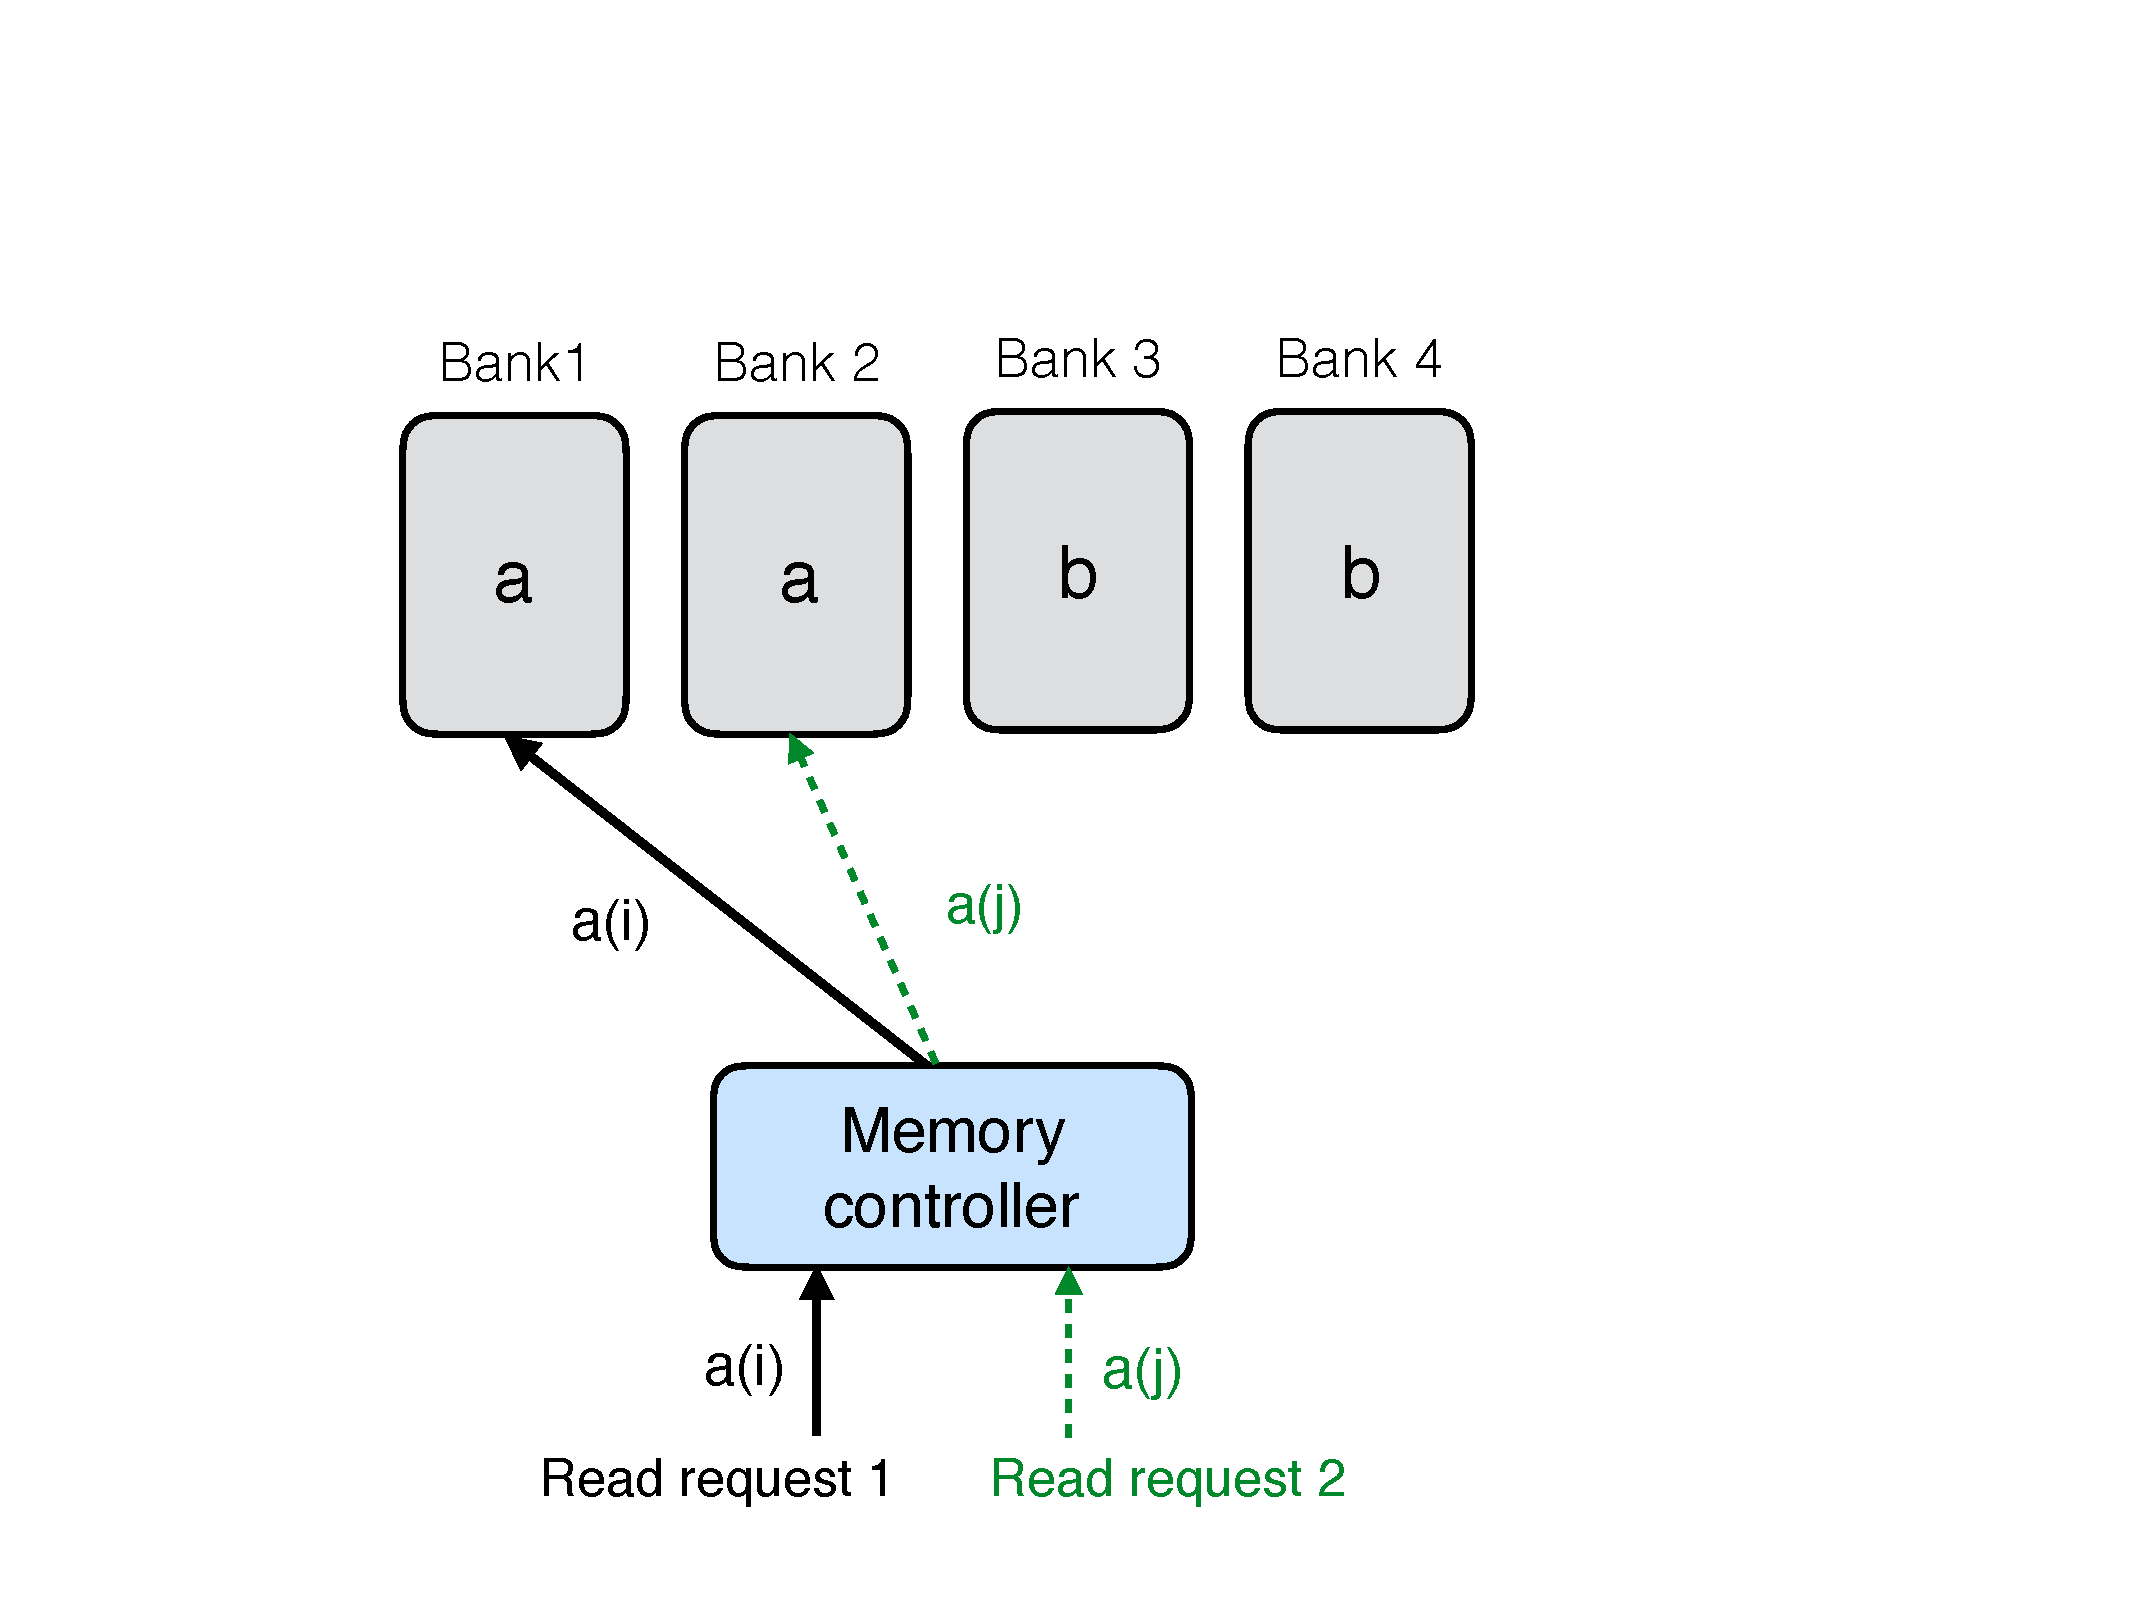
\includegraphics[width=0.425\linewidth]{fig/read-replication.pdf}
\caption{$2$-replication based design to support multiple $2$ read requests in the same memory clock cycle. The two banks' worth of data $\mathbf{a} = [a(1),\ldots, a(L)]$ and $\mathbf{b} = [b(1),\ldots, b(L)]$, all the data elements are stored on two distinct memory banks. Note that any $2$ read requests to distinct memory banks. For example, the figure considers the scenario with $2$ read requests for elements $\{a(i), a(j)\}$. Since both $a(i)$ and $a(j)$ are stored on $2$ banks, one of those banks can be used to serve each request without causing any bank conflicts. It's straightforward to verify that this memory design avoids bank conflicts for any other set of $2$ read requests.}
\label{fig:read_replication}
\end{figure}
%---------------------------

%---------------------------
\begin{figure}[t!]
\centering
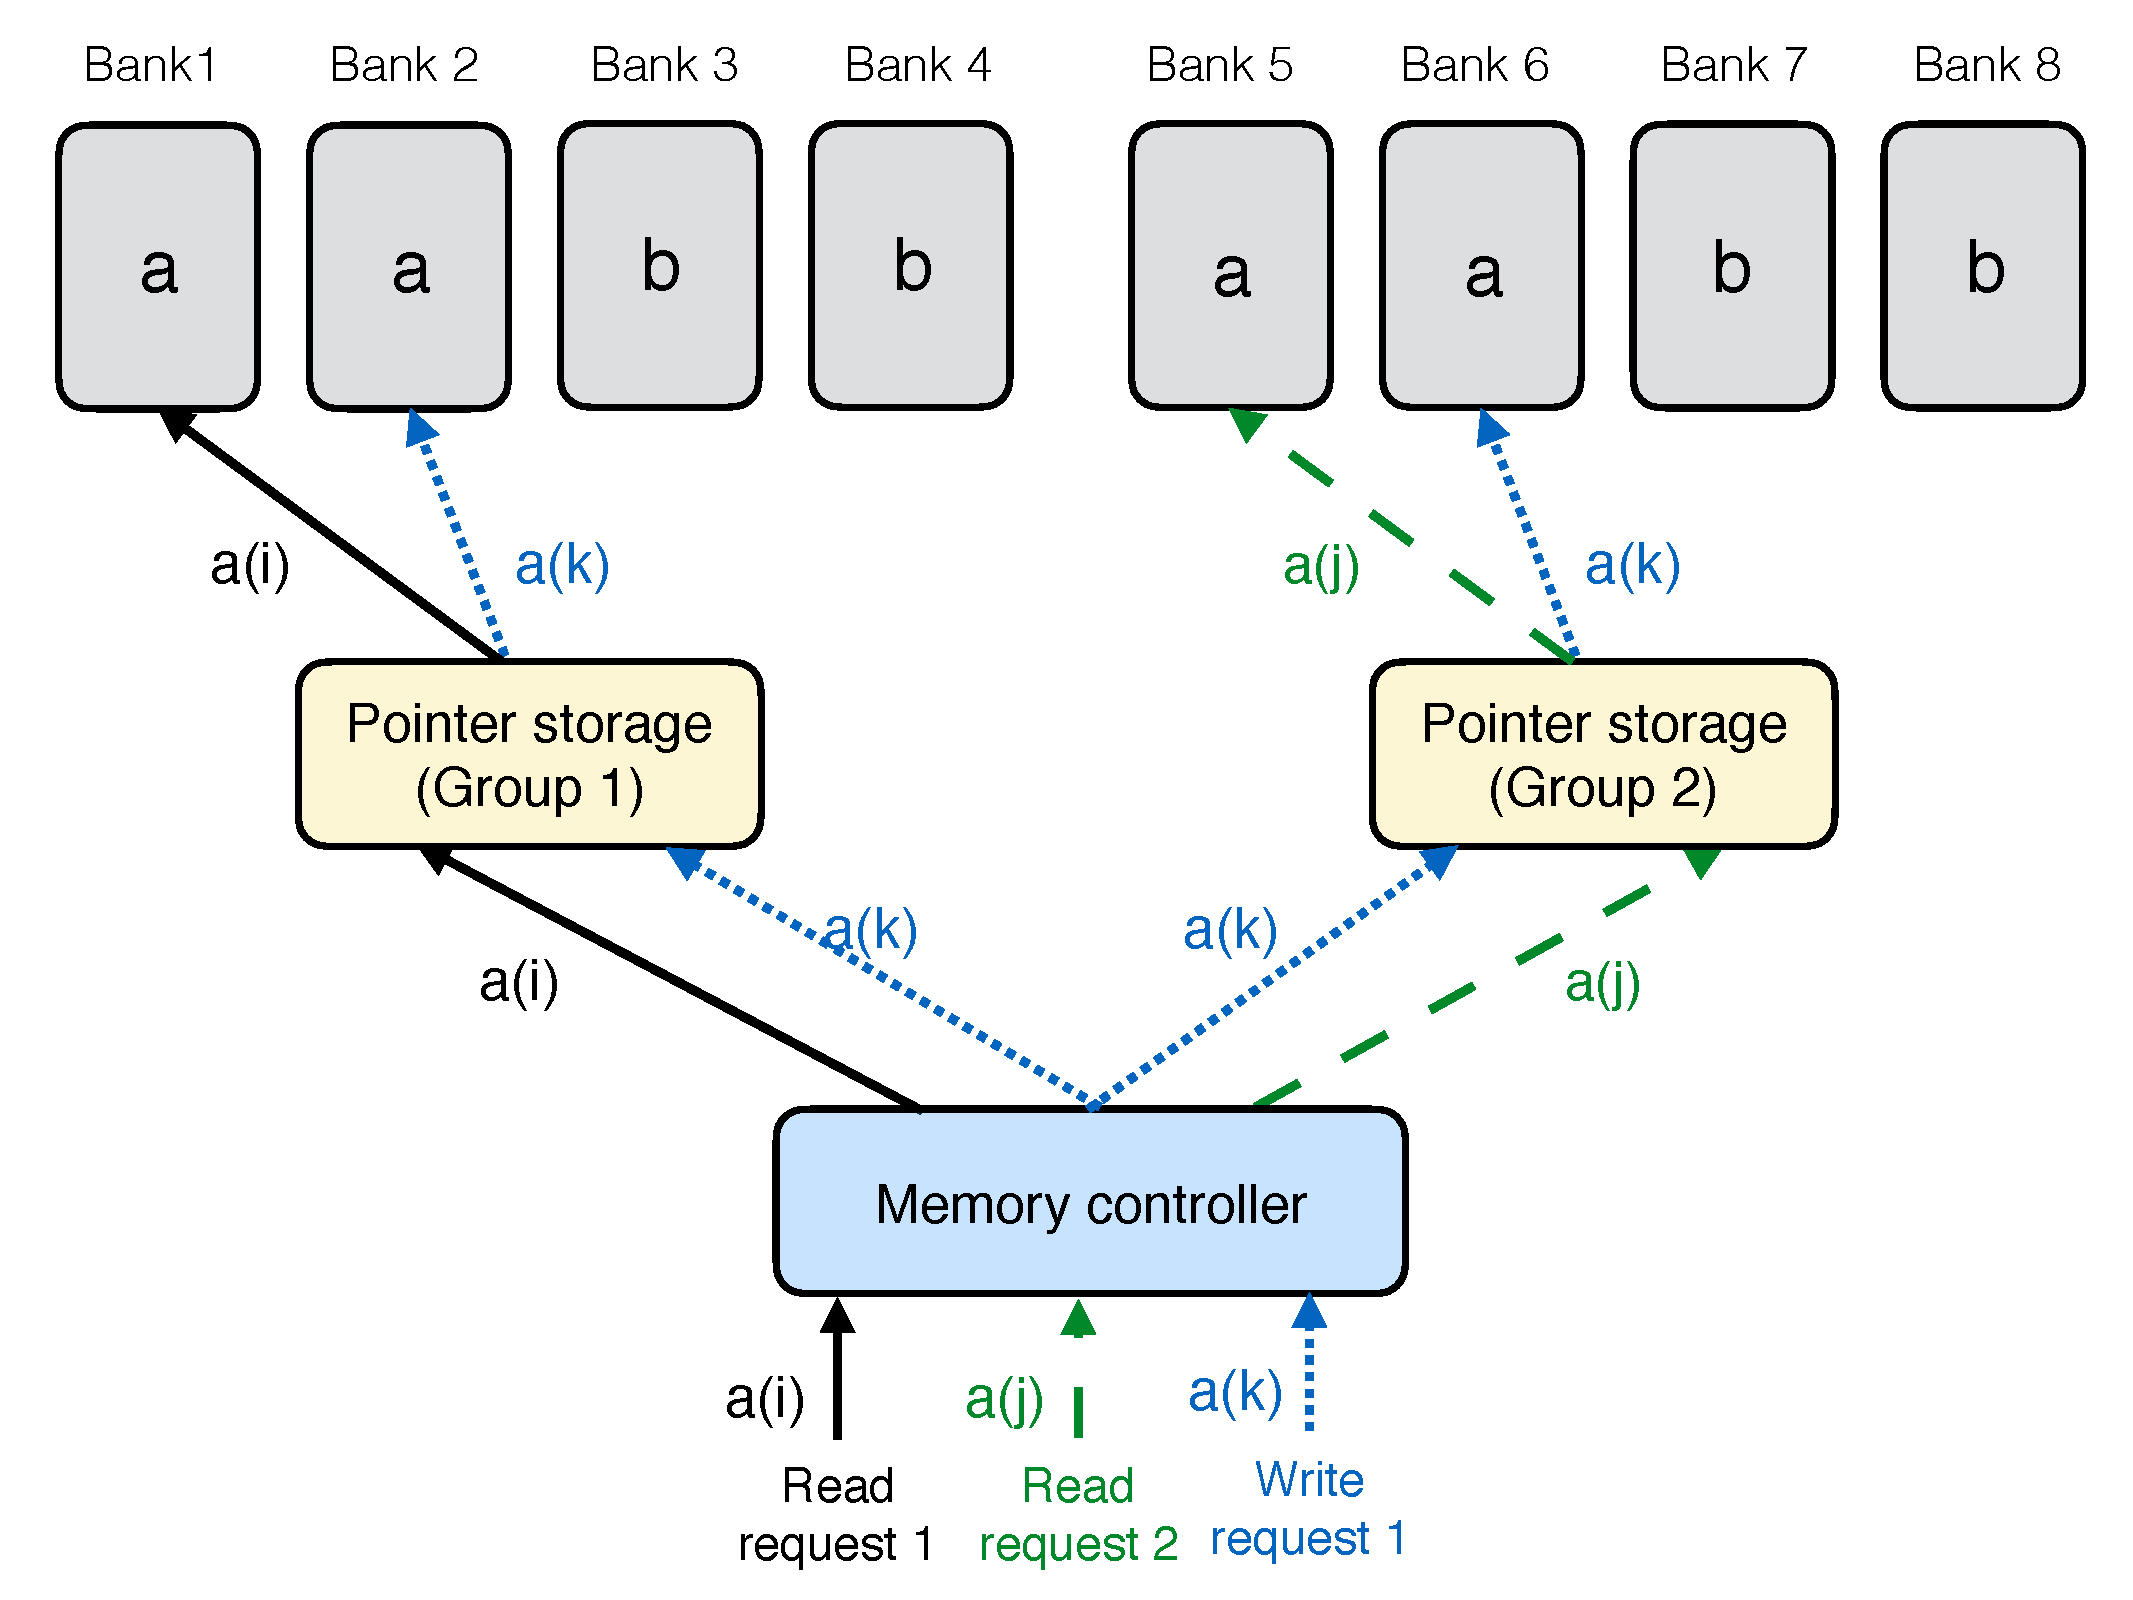
\includegraphics[width=0.86\linewidth]{fig/rw-replication.pdf}
\caption{$4$-replication based design to support $r = 2$ read requests and $w = 1$ write request in one memory clock cycle. Both collections of information elements $\mathbf{a} = [a(1),\ldots, a(L)]$ and $\mathbf{b} = [b(1),\ldots, b(L)]$ are replicated on $r\cdot (w + 1) = 4$ different single-port memory banks. These banks are then partitioned into $r = 2$ disjoint groups. We utilize each group to serve one read request. In a given memory clock cycle, we focus on the specific access pattern with the read requests for $\{a(i), a(j)\}$ and the write request for $\{a(k)\}$. Assuming that Bank $1$ (from Group $1$) and Bank $5$ (from Group $2$) have the updated versions of the data elements $a(i)$ and $a(j)$, respectively, we serve the read requests for $a(i)$ and $a(j)$ from Bank $1$ and Bank $5$, respectively. As for the write request for the data element $a(k)$, we need to perform this write request in at least one memory bank in each of the two groups. This will enable both groups to continue serving any possible set of $r = 2$ read requests during future accesses. Since we have one memory bank storing $a(k)$ in each of the groups that is not busy serving write request, we write the updated $a(k)$ in these non-busy banks (Bank $2$ and Bank $3$ in this case). During the writing process, we also need to modify the pointer storage accordingly to keep track of the banks in each group that are storing the most updated values of different data elements.}
\label{fig:rw_replication}
\end{figure}
%---------------------------
\subsubsection{Read and Write Support}
\label{sec:rw}
\Ankit{Mainly describing the results from the work of Auerbach, Chen, and  Paul\cite{ACP88}.} 
% It is evident from the discussion so far that we can indeed emulate the behavior of a multi-port memory on read requests by storing data on single-port memory banks in a redundant manner. 
The redundancy mechanism can vary from simple replication-based strategy to more sophisticated coding schemes. However, a successful memory design necessarily need to address the issues of (potentially multiple) write requests as well. A challenge that arises in the presence of write requests is that one also need to ensure consistency across different requests. This requires managing multiple versions of the same information across all the memory banks and making sure that stale information is not supplied in response to a particular read request. 

Restricting ourselves to replication-based designs, a multi-port memory that simultaneously supports $r$ read requests and $w$ write requests in a memory cycle can be emulated by  using a $r\cdot(w + 1)$ replication scheme, where $r\cdot(w+1)$ copies of each data element are stored on $r\cdot(w + 1)$ different single-port memory banks. We illustrate this scheme for $r = 2$ and $w = 1$ in Figure~\ref{fig:rw_replication}. According to all of our previous illustrations, we assume that we have two symbols' worth of information $\mathbf{a} = [a(1),\ldots, a(L)]$ and $\mathbf{b}  = [b(1),\ldots, b(L)]$. We store $4$ copies each of data elements $\mathbf{a}$ and $\mathbf{b}$ and partition the banks that store a data element into $r = 2$ disjoint groups with each group containing $(w + 1) = 2$ memory banks. In Figure~\ref{fig:rw_replication}, Banks $1$ -- $4$ and Banks $5$ -- $8$ correspond to Group $1$ and Group $2$, respectively. For the underlying replication-based scheme, we also require additional storage space to keep track of the versions of different copies of the information elements. This space is referred to as the pointer storage. In Figure~\ref{fig:rw_replication}, we illustrate how this design serves a particular set of $2$ read requests and $1$ write request.\\


%\subsection{Better emulation of multi-port memories}
\subsection{Storage-efficient emulation of multi-port memories}
\label{sec:efficient_emulation}

As described in Section~\ref{sec:emulation}, introducing redundancy to systems which use single-port memory banks allows such systems emulate the behavior of multi-port banks. In a setup where multi-port reads are supported (cf. Section~\ref{sec:read_only}) such emulation has little computational and storage cost. Emulating multi-port read and write systems is more costly (cf. Section~\ref{sec:rw}). A greater number of single-port memory banks are needed, and systems which redundantly store memory require tracking of the various versions of the data elements present in the memory banks. Furthermore, the presence of varying version of elements in the banks complicates the process of arbitration, as some memory banks may contain stale elements. Many programs in multi-core environments involve significant numbers of write requests, so any system which emulates multi-port memory using single-port memory must take these complications into account.

{\color{red}We believe that various tasks that arise in the presence of write requests and contribute to computational overhead of the memory design, including synchronization among memory banks and complicated arbitration, can be better managed at the algorithmic level.\Ethan{good point!} Note that these tasks are performed at memory controller. It is possible to reduce the effect of these tasks on the overall performance of memory system by relying on the increasing available computational resources while designing the memory controller. On the other hand, we believe that the storage overhead is a more fundamental issue that needs to be addressed for the emulation of the multi-port memories to be viable and appealing. In particular, the large replication factor in a naive design limits the applicability of the obtained memory in practice due to large storage overhead and the associated large area requirement resulting from this.}

In order to reduce the storage overhead incurred by multi-port emulation, we avoid the native two-step memory design. Another approach arises from the observation that some data banks are often left unused during arbitration in individual memory cycles, while other data banks receive multiple requests. We encode the elements of the data banks using specific coding schemes to generate parity banks. Elements drawn from multiple data banks are encoded and stored in the parity banks. This approach allows us to utilize unused data banks to decode elements stored in the parity banks in service of the heavily requested data banks. We recognize that this approach leads to increased complexity at the memory controller. {\color{red} {\em However, we show that the increment in the complexity can be kept within the acceptable level while insuring storage-efficient emulation of multi-port memories with the help of better algorithmic design.}}

\subsection{Related work}

Coding theory is one of the well studied field which deals with mitigating the adversarial effects of the underlying medium in an information processing system~\cite{MacSlo, Cover}. In particular, the developments in the field have enabled both reliable communication across noisy channel and storage over fault-prone storage units in resource efficient manners. Recently, we have witnessed intensive efforts towards the applications of coding theoretic ideas to design large scale distributed storage systems~(see e.g., \cite{Azure, SAPDVCB13, Rashmi14}). In this domain of coding for distributed storage systems, the issue of access efficiency has also received attention, especially the ability to support multiple simultaneous read accesses with small storage overhead~\cite{batchcodes, RPDV16, RSDG16, Wang2017} and references therein. In this paper, we rely on the coding techniques developed under in this domain to realize emulation of multi-port memories using single-port memory banks. However, we note that the existing work on batch codes~\cite{batchcodes} only focuses on the read requests. On the other hand, the successful emulation of multi-port memory also requires handling write requests in an efficient manner. Furthermore, the design presented in this paper also needs to address the entire memory system which also involves memory controller design as opposed to just focusing on the storage array. 


Here, we note that the issue of designing coding schemes that have low update complexity, \textit{i.e.} that can be modified with low overhead as the information gets updated, have also received some attention in the literature (see e.g.,~\cite{ASV10, MCW14}). However, this treatment is extensive enough to address the update issues that arise in the context of our memory systems, where write requests may be very frequent and a large portion of the bank array needs to get updated. Again, the key issue that distinguish our work from the majority of the literature on coding for distributed storage is that we need to take the interplay among read and write requests and its effect on the overall performance (latency) into account.\Ethan{good point} Furthermore, we  are not allowed to encode across a very large number of storage units (memory banks in our case), which is very much feasible in today's large scale cloud storage systems.

In this paper, we also explore the idea of proactively prefetching the information from memory banks to improve the access efficiency of our memory design. The idea of prefetching in realizing fast data transfer between processors and memory has been previously explored in the literature (see \cite{Kim2016, Kadjo2014, Shevgoor2015, JL2013} and references therein). 
%However, our work addresses the issue of data prefetching in the context of coded memory system which is not addressed earlier in the literature. 
More recently, an LSTM-based recurrent neural network was used to predict future memory access requests on the SPEC 2006 benchmark dataset \cite{lstm2018}. This deep learning method may be used in addition to our proposed frequency-based approach.
Our combination of coded memory and prefetching also shares some similarity with the recent line of work on coded caching~\cite{MN16a} which aims to reduce the data downloaded from servers in a communication network by utilizing the cache available at the end users. Here, we would like to point out that there are many key differences in the our setup with coded memory banks with that considered in \cite{MN16a}. Our setup has data stored in an encoded form stored across memory banks and caching is enabled by the memory controller, which is a centralized unit. In contrast, the setup of coded caching has a centralized storage system (server) and cache units that store encoded information distributed across users.

{\color{red} {\bf The work which is closest to our solution for emulating a multi-port memory is by Iyer and Chuang~\cite{Memoir_xor, Memoir_xor_virtual}, where they also employ XORing based coding schemes to redundantly store information in an array of single-port memory banks. However, we note that our work significantly differers from \cite{Memoir_xor, Memoir_xor_virtual} as we specifically rely on different coding schemes arising under the framework of batch codes~\cite{batchcodes}. Additionally, due to the employment of distinct coding techniques, the design of memory controller in our work also differs from that in \cite{Memoir_xor, Memoir_xor_virtual}.}}

\Ankit{Also cite the work by Rivest et al.~\cite{RG91} and Endo, Matsumura and Yamada~\cite{EMY91}.}

%\section{Motivation}
%
%\subsection{Dual port RAM}
%
%\subsubsection{Replication}
%Because the size of the dual-ported SRAM bit-cell is almost double that of the single-ported SRAM bit-cell, a more versatile way (i.e., can do 2 reads in one cycle or one write) to implement dual-ported SRAM is by duplicating SRAM banks, as shown in Figure 3. In this way the bandwidth does not suffer from any loss for performing 2 simultaneous read operations, but only suffers 1 arbitration loss when performing simultaneous read and write operations (i.e., cannot perform 1 read and 1 write in the same cycle). The area is similar to that used in dual-ported circuit implementations. The advantage of this implementation is simplicity while the disadvantage is that if frequent write access is required the performance (bandwidth) is not as good as the true 1R1W SRAMs which can do a simultaneous read and write in one cycle.
%
%\subsubsection{Replication with pointer storage}
%
%Replication scheme $r + w$ replications...for $rRwW$ multipart memory.
%
%\subsubsection{Bank interleaving and arbitration}
%
%Another alternative is to use bank interleaving and arbitration circuits to allow for simultaneous access of different banks of memory. Occasional stalls are necessary in this approach if the arbitration circuit finds conflicting access to the same memory banks. Its operation is illustrated in Figure 4.
%
%Figure 4. Multiple accesses to SRAM by Bank interleaving with lower address bits. A large SRAM bank is sub-divided into n (n ? 2) smaller single-ported SRAM banks to support 2 or more simultaneous accesses. An arbitration unit is used in case conflicting addresses want to access the same bank, in which case one of the accesses is delayed.
%
%
%
%
%{\color{red}
%SRAMs can be categorized as single-ported or multi-ported. The single-ported SRAM is the most common type of SRAM with the best area efficiency and is used for most compiler memories due to its modular approach. Multi-ported memories are either not area efficient or with limited storage capability. Logical implementation of multi-ported memories with interleaved banks can be area efficient (because there is no memory duplication), but requires arbitration and flow-control circuits. Duplicating single-ported memory banks can support 2 reads and 1 write type of accesses with no additional delays and 1 read and 1 write type of access with 1.5 times the delay of read access;  Also its size is competitive relative to the true dual-ported memories. True multi-ported memories can be implemented with single-ported memories by replicating the memories multiple times. The area cost is r(w+1) times the number of bank replications.  Algorithmic approaches of multi-port memory design (such as Memoir) include caches and different ways of buffering of read and write data, with advantages being area efficiency and disadvantages including design complexity. Algorithmic memories can be statistical with lower areas or deterministic with higher areas, depending on the application.}

